\section{Arquitetura e Gerenciamento de Recursos no Zephyr}

A arquitetura do Zephyr fundamenta-se em princípios de alta modularidade, permitindo que o sistema seja escalonado com precisão para diferentes aplicações. Por meio do sistema de configuração \textit{Kconfig}, é possível compilar estritamente os componentes necessários do \textit{kernel}, o que otimiza significativamente o uso da memória em dispositivos restritos. 

Para o gerenciamento de \textit{hardware}, o sistema adota a \textit{Devicetree}, uma estrutura hierárquica de dados introduzida pelo ecossistema Linux que descreve os componentes físicos do microcontrolador de forma totalmente independente do código-fonte da aplicação. Essa abstração confere alta portabilidade, pois a migração entre diferentes placas ou arquiteturas exige apenas a reconfiguração dos arquivos descritivos. Diferentemente de sistemas que resolvem \textit{hardware} em tempo de execução, o Zephyr utiliza o compilador de \textit{Devicetree} (DTC) para converter os arquivos de descrição (organizados em nós, propriedades e identificadores \textit{compatible}) em macros da linguagem C durante o processo de \textit{build}, conforme ilustrado na \autoref{fig:devicetree_fluxo}. Essa abordagem garante um \textit{overhead} nulo de processamento durante a execução e permite uma validação rigorosa dos pinos e periféricos em tempo de compilação \cite{zephyr_dt}.

\begin{figure}[htb]
    \centering
    \caption{Fluxo de compilação da Devicetree no Zephyr OS, ilustrando a conversão de nós hierárquicos em macros C.}
    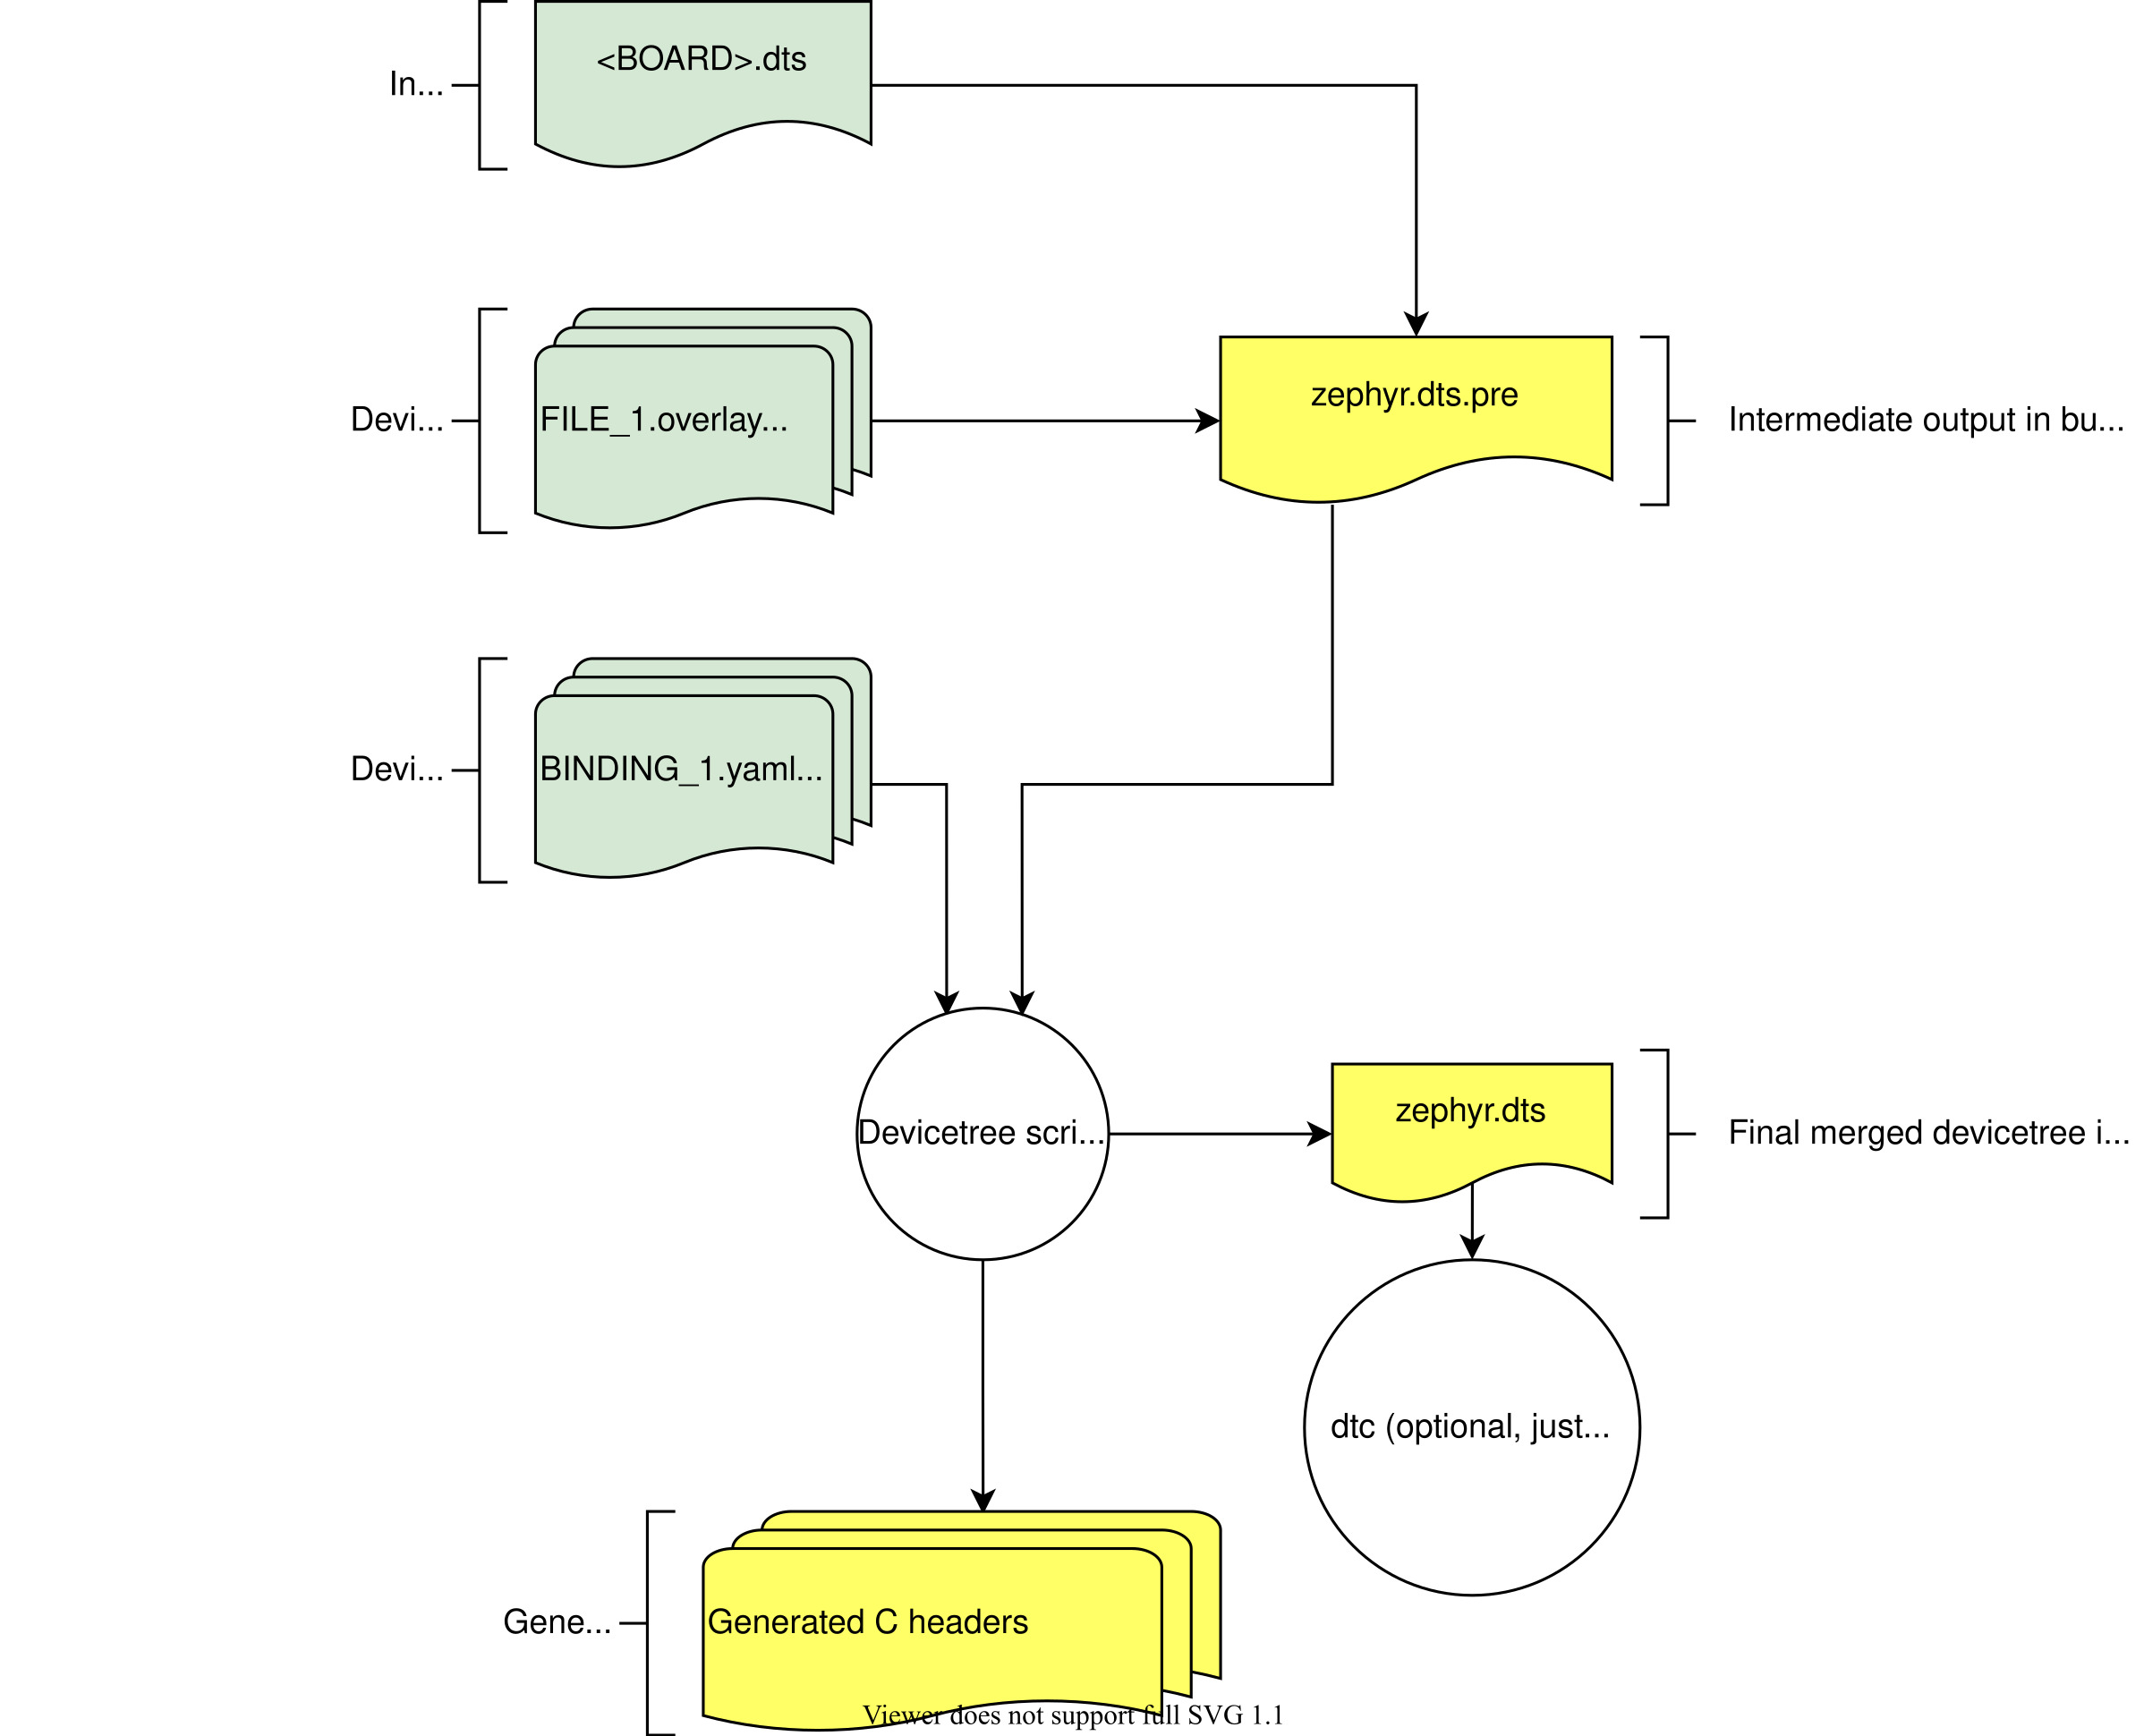
\includegraphics[width=0.7\textwidth]{Textuais/Imgs/Revisao/zephyr_dt_inputs_outputs.jpg}
    \label{fig:devicetree_fluxo}
    \fonte{\cite{zephyr_dt}.}
\end{figure}

No que tange à execução e concorrência, o Zephyr é estruturado em torno de um modelo multitarefa, gerenciando \textit{threads} por meio de um escalonador determinístico. O sistema suporta tanto \textit{threads} cooperativas — que cedem o controle voluntariamente — quanto preemptivas. O \textit{kernel} organiza essas tarefas dividindo o espaço de prioridades: valores negativos são estritamente atribuídos a \textit{threads} cooperativas, protegendo-as de preempção por tempo (\textit{time-slicing}), enquanto valores não-negativos destinam-se às \textit{threads} preemptivas. O ciclo de vida dessas tarefas é gerido por uma máquina de estados rigorosa, ilustrada na \autoref{fig:thread_states}, onde uma \textit{thread} transita entre estados como Pronto (\textit{Ready}), Em Execução (\textit{Running}), Bloqueado (\textit{Waiting}/\textit{Blocked}) por recursos ou eventos, e Suspenso (\textit{Suspended}) \cite{zephyr_threads}.


Para que essas múltiplas \textit{threads} operem de forma harmônica e segura, o \textit{kernel} fornece uma API nativa para Comunicação Interprocessos (IPC, do inglês \textit{Inter-Process Communication}). Através de mecanismos de sincronização e troca de mensagens, como semáforos, \textit{mutexes}, filas de mensagens (\textit{message queues}) e \textit{pipes}, o RTOS garante a integridade dos dados compartilhados e previne condições de corrida, estabelecendo um ambiente robusto e previsível para o processamento de sistemas embarcados \cite{zephyr_ipc}.

\begin{figure}[H]
    \centering

     \caption{Máquina de estados simplificada das \textit{threads} no Zephyr, demonstrando as transições de ciclo de vida gerenciadas pelo escalonador.}
    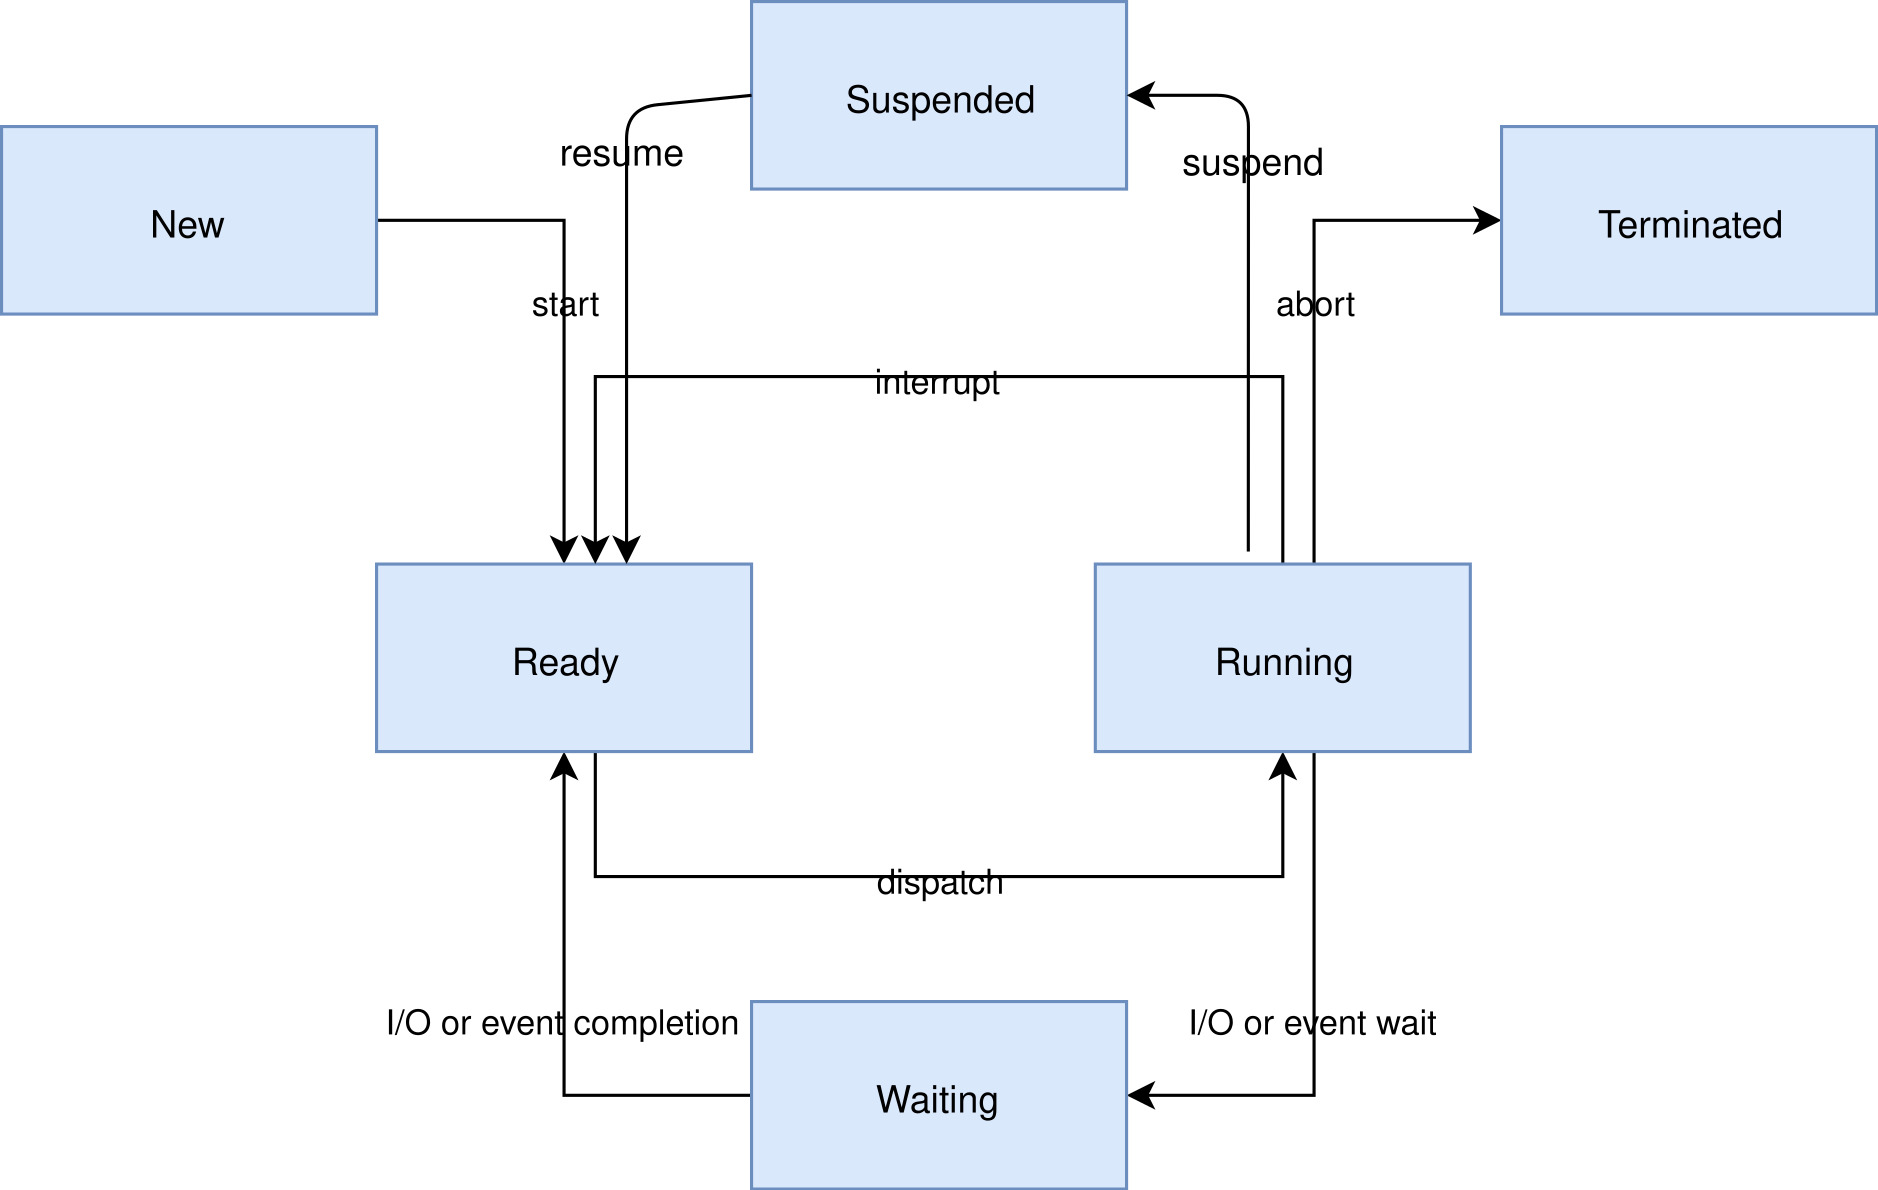
\includegraphics[width=0.7\textwidth]{Textuais/Imgs/Revisao/Zephyr_thread_states.jpg}
    \label{fig:thread_states}
    \fonte{\cite{zephyr_threads}.}
\end{figure}
